\documentclass[tikz,border=8pt]{standalone}
% Shared look for every TikZ diagram. Load with \input{../../tools/tikz-style.tex}
\usepackage[T1]{fontenc}
\usepackage{lmodern}
\renewcommand{\sfdefault}{lmr}  % diagrams use the same serif as the text
\usetikzlibrary{arrows.meta, positioning, shapes.geometric, calc, fit, backgrounds}
\definecolor{cblue}{HTML}{4C78A8}
\definecolor{corange}{HTML}{F58518}
\definecolor{cgreen}{HTML}{54A24B}
\definecolor{cred}{HTML}{E45756}
\definecolor{cpurple}{HTML}{B279A2}
\definecolor{cgrey}{HTML}{6B6B6B}
\tikzset{
  every picture/.style={font=\sffamily, line width=1.2pt},
  box/.style={draw=#1, fill=#1!12, rounded corners=4pt, align=center, inner sep=7pt, minimum height=1.1cm},
  box/.default=cgrey,
  arrow/.style={-{Stealth[length=3mm]}, draw=cgrey, line width=1.4pt},
  title/.style={font=\sffamily\bfseries\Large},
  note/.style={font=\sffamily\small, text=cgrey, align=center},
}
\AtBeginDocument{\hyphenpenalty=10000 \exhyphenpenalty=10000}

\begin{document}
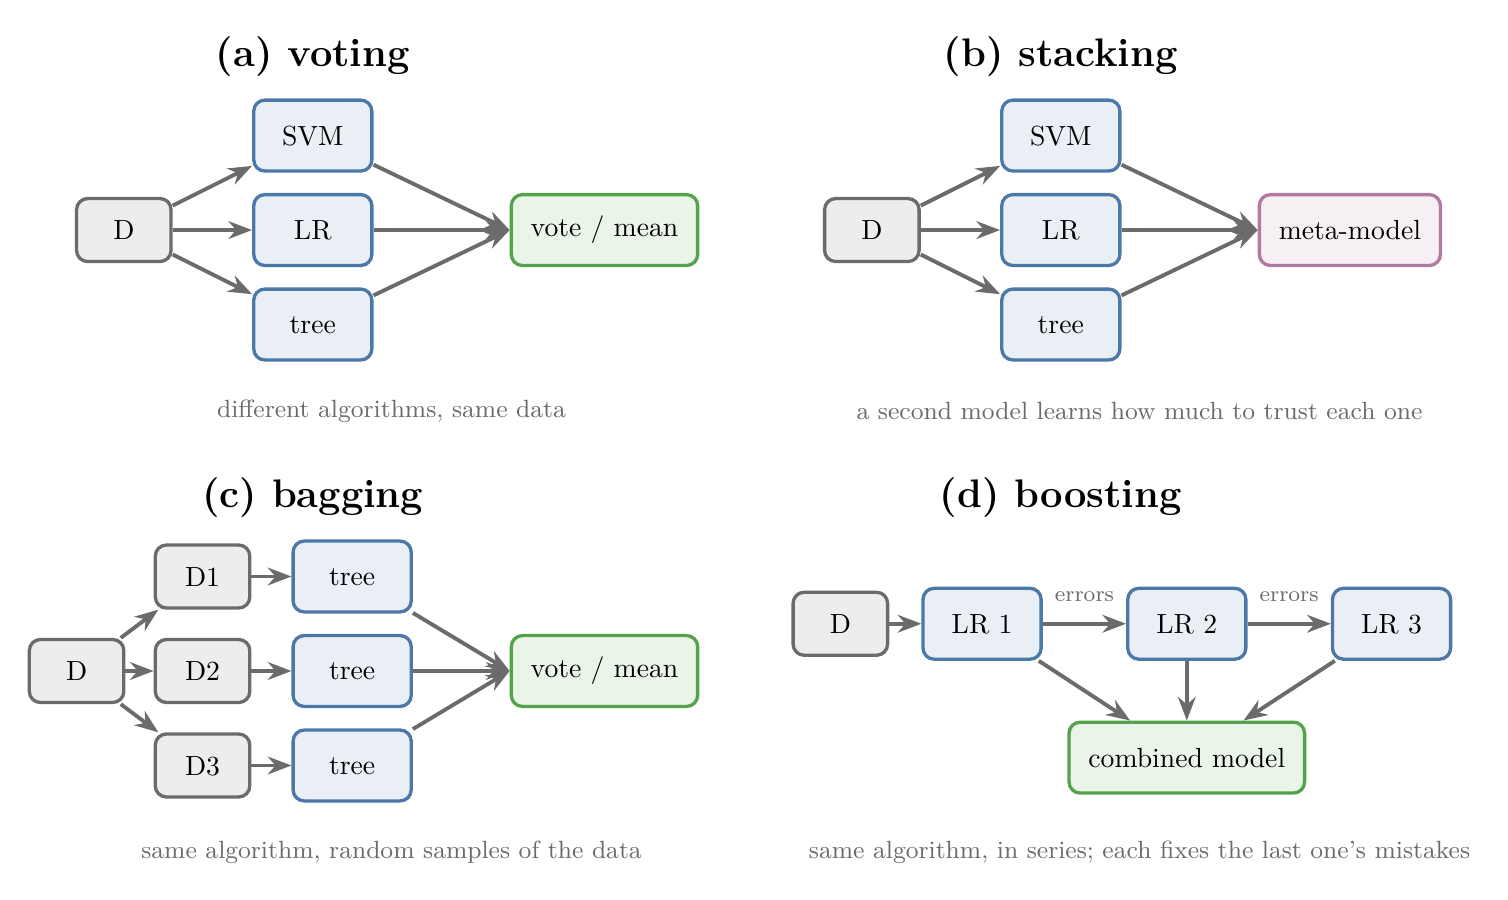
\begin{tikzpicture}[
  m/.style={box=cblue, minimum width=1.5cm, minimum height=0.9cm},
  s/.style={box=cgrey, minimum width=1.2cm, minimum height=0.8cm},
  o/.style={box=cgreen, minimum width=2.3cm, minimum height=0.9cm},
  k/.style={box=cpurple, minimum width=2.3cm, minimum height=0.9cm}]
  % ---------- (a) voting
  \begin{scope}
  \node[title] at (2.4,2.2) {(a) voting};
  \node[s] (D) at (0,0) {D};
  \node[m] (a1) at (2.4,1.2) {SVM};
  \node[m] (a2) at (2.4,0) {LR};
  \node[m] (a3) at (2.4,-1.2) {tree};
  \foreach \i in {1,2,3} {\draw[arrow] (D) -- (a\i); \draw[arrow] (a\i) -- (4.9,0);}
  \node[o, anchor=west] at (4.9,0) {vote / mean};
  \node[note] at (3.4,-2.3) {different algorithms, same data};
  \end{scope}
  % ---------- (b) stacking
  \begin{scope}[xshift=9.5cm]
  \node[title] at (2.4,2.2) {(b) stacking};
  \node[s] (D) at (0,0) {D};
  \node[m] (b1) at (2.4,1.2) {SVM};
  \node[m] (b2) at (2.4,0) {LR};
  \node[m] (b3) at (2.4,-1.2) {tree};
  \foreach \i in {1,2,3} {\draw[arrow] (D) -- (b\i); \draw[arrow] (b\i) -- (4.9,0);}
  \node[k, anchor=west] at (4.9,0) {meta-model};
  \node[note] at (3.4,-2.3) {a second model learns how much to trust each one};
  \end{scope}
  % ---------- (c) bagging
  \begin{scope}[yshift=-5.6cm]
  \node[title] at (2.4,2.2) {(c) bagging};
  \node[s] (D) at (-0.6,0) {D};
  \node[s] (c1s) at (1.0,1.2) {D1};
  \node[s] (c2s) at (1.0,0) {D2};
  \node[s] (c3s) at (1.0,-1.2) {D3};
  \node[m] (c1) at (2.9,1.2) {tree};
  \node[m] (c2) at (2.9,0) {tree};
  \node[m] (c3) at (2.9,-1.2) {tree};
  \foreach \i in {1,2,3} {\draw[arrow] (D) -- (c\i s); \draw[arrow] (c\i s) -- (c\i); \draw[arrow] (c\i) -- (4.9,0);}
  \node[o, anchor=west] at (4.9,0) {vote / mean};
  \node[note] at (3.4,-2.3) {same algorithm, random samples of the data};
  \end{scope}
  % ---------- (d) boosting
  \begin{scope}[xshift=9.5cm, yshift=-5.6cm]
  \node[title] at (2.4,2.2) {(d) boosting};
  \node[s] (D) at (-0.4,0.6) {D};
  \node[m] (d1) at (1.4,0.6) {LR 1};
  \node[m] (d2) at (4.0,0.6) {LR 2};
  \node[m] (d3) at (6.6,0.6) {LR 3};
  \draw[arrow] (D) -- (d1);
  \draw[arrow] (d1) -- node[above=4pt, note, font=\sffamily\footnotesize] {errors} (d2);
  \draw[arrow] (d2) -- node[above=4pt, note, font=\sffamily\footnotesize] {errors} (d3);
  \node[o] (dout) at (4.0,-1.1) {combined model};
  \foreach \i in {1,2,3} \draw[arrow] (d\i) -- (dout);
  \node[note] at (3.4,-2.3) {same algorithm, in series; each fixes the last one's mistakes};
  \end{scope}
\end{tikzpicture}
\end{document}
